\subsection{Formula-size analysis}
Let $a_E(k)$ and $c_E(k)$ count generated auxiliary variables and clauses
for one $k$-input AMO under encoding $E$. Both counts are zero for $k\le1$.
The direct counts are
\begin{align}
(a_{\mathrm{pair}},c_{\mathrm{pair}})&=(0,\tbinom{k}{2}),\\
(a_{\mathrm{bin}},c_{\mathrm{bin}})&=(\lceil\log_2 k\rceil,
k\lceil\log_2 k\rceil),\qquad k\ge3,\\
(a_{\mathrm{seq}},c_{\mathrm{seq}})&=(k-1,3k-4),\qquad k\ge3.
\end{align}
For both binary and sequential $k=2$ the counts are $(0,1)$.
For both commander and
product, $k\le4$ uses the pairwise counts. For larger commander groups,
with $t_j=|G_j|$ and $m=\lceil k/3\rceil$, the implementation gives
\begin{align}
a_{\mathrm{cmd}}(k)&=m+a_{\mathrm{cmd}}(m),\\
c_{\mathrm{cmd}}(k)&=\sum_{j=1}^m\tbinom{t_j}{2}+k+m+c_{\mathrm{cmd}}(m).
\end{align}
The terms count within-group pairs, $k$ forward clauses, $m$ reverse
clauses, and recursive commander AMO. For product, with $p,q$ as above,
\begin{align}
a_{\mathrm{prod}}(k)&=p+q+a_{\mathrm{prod}}(p)+a_{\mathrm{prod}}(q),\\
c_{\mathrm{prod}}(k)&=2k+c_{\mathrm{prod}}(p)+c_{\mathrm{prod}}(q).
\end{align}
These are counts for the actual recursive implementation; in particular,
no unused-cell clauses enter the product recurrence.

For $n\ge2$, there are $2n$ row and column AMO groups of length $n$.
Across the two diagonal directions, there are two more groups of length
$n$ and four of each length $2,\ldots,n-1$. Thus the total variables and
minimal-formulation clauses are
\begin{align}
V_E(n)&=n^2+(2n+2)a_E(n)+4\sum_{k=2}^{n-1}a_E(k),\label{eq:size-vars}\\
C_{E,\min}(n)&=n+(2n+2)c_E(n)+4\sum_{k=2}^{n-1}c_E(k).
\label{eq:size-clauses}
\end{align}
The initial $n$ clauses are row ALO. Extended adds exactly $n$ column
ALO clauses, giving $C_{E,\mathrm{ext}}=C_{E,\min}+n$ and the same $V_E$.
For $n=1$, the counts are one variable and one minimal clause; extended
generates a second, duplicate ALO clause. Counts refer to emitted clauses,
before any solver simplification.

\begin{table}[pos=htbp]
\centering\small
\caption{Asymptotic size of the complete board CNF, derived from the
implemented AMO constructions. Both formulations have these orders.}
\label{tab:amo}
\begin{tabular}{lrr}\toprule
Encoding & Auxiliary variables & Clauses\\\midrule
Pairwise & 0 & $\Theta(n^3)$\\
Binary & $O(n\log n)$ & $O(n^2\log n)$\\
Commander & $O(n^2)$ & $O(n^2)$\\
Recursive product & $O(n^{3/2})$ & $O(n^2)$\\
Sequential counter & $O(n^2)$ & $O(n^2)$\\\bottomrule
\end{tabular}
\end{table}

For pairwise, substituting $c(k)=\binom{k}{2}$ yields
\begin{equation}
C_{\mathrm{pair},\min}(n)
=\frac{5n^3-6n^2+4n}{3},\qquad n\ge2.
\end{equation}
As a concrete check, a minimal $4\times4$ board has 16 variables and
80 clauses: four row ALO clauses, 48 row/column pair clauses, and
28 diagonal pair clauses. Extended has 84 clauses.
Figure~\ref{fig:sizes} plots the exact counts for the six encoding-study
sizes. Counts are computed even when a timed run was unfinished.
\begin{figure}[pos=htbp]
\centering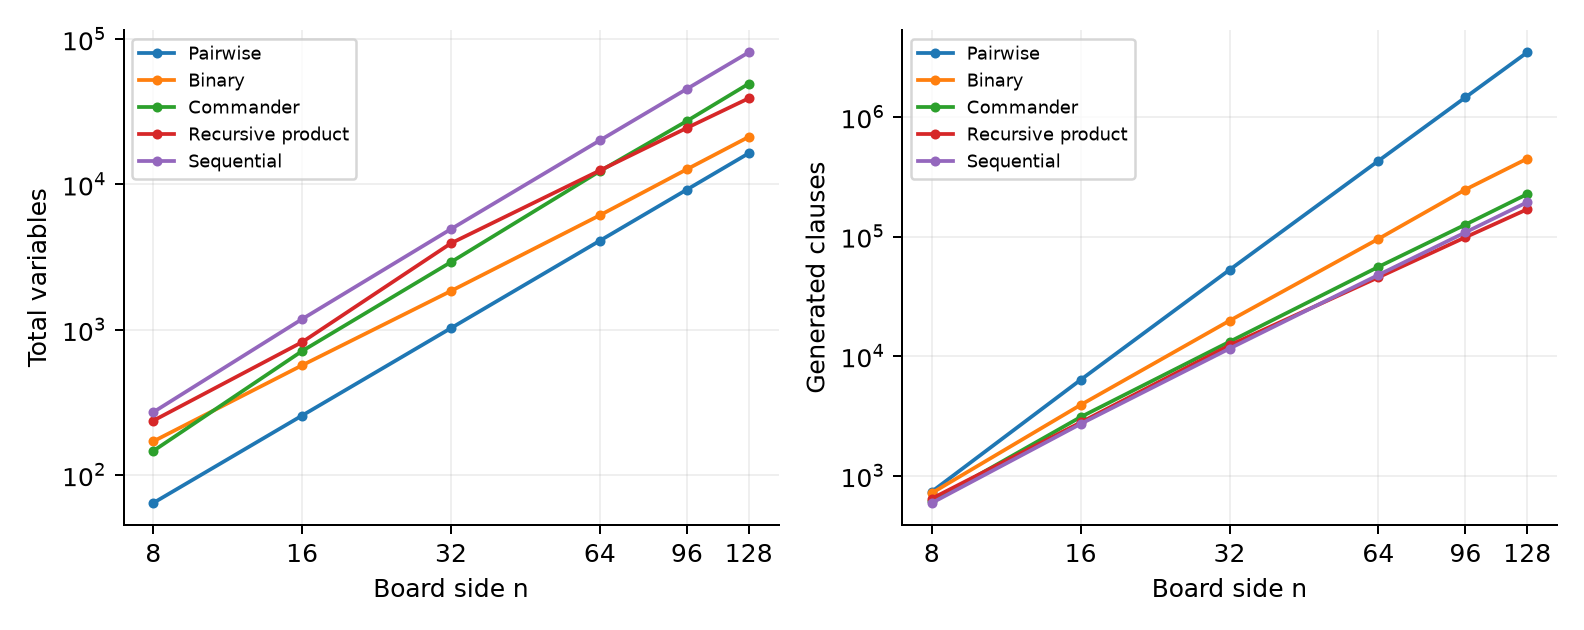
\includegraphics[width=.95\linewidth]{figs/formula_sizes.png}
\caption{Exact generated CNF size for the minimal formulation. Both axes
are logarithmic; total variables include board variables and auxiliaries.
The curves describe construction size, not measured runtime.}
\label{fig:sizes}
\end{figure}
\FloatBarrier
The recursive product and commander constructions reduce clause growth,
but their auxiliaries and propagation paths differ. The experiments
therefore compare size with measured construction and search costs
rather than treating the smallest CNF as the fastest solver configuration.
